% compila con pdflatex
\documentclass[10pt]{article}
\usepackage[margin=1.2cm,landscape]{geometry}
\usepackage{tikz}
\usetikzlibrary{shapes.geometric, arrows.meta, positioning, fit}
\pagestyle{empty}

% estilos compactos
\tikzset{
  box/.style={rectangle, rounded corners, draw, align=left,
    minimum width=36mm, minimum height=6mm, font=\scriptsize, inner sep=2mm},
  startstop/.style={ellipse, draw, align=center,
    minimum width=30mm, minimum height=7mm, font=\scriptsize, inner sep=2mm},
  dec/.style={diamond, draw, aspect=2, align=center, font=\scriptsize, inner sep=1.2mm},
  line/.style={-{Latex}, thick},
  note/.style={draw, dashed, rounded corners, inner sep=1.5mm, font=\tiny}
}

\begin{document}
\centering

% ajusta toda la figura al ancho disponible
\resizebox{\linewidth}{!}{%
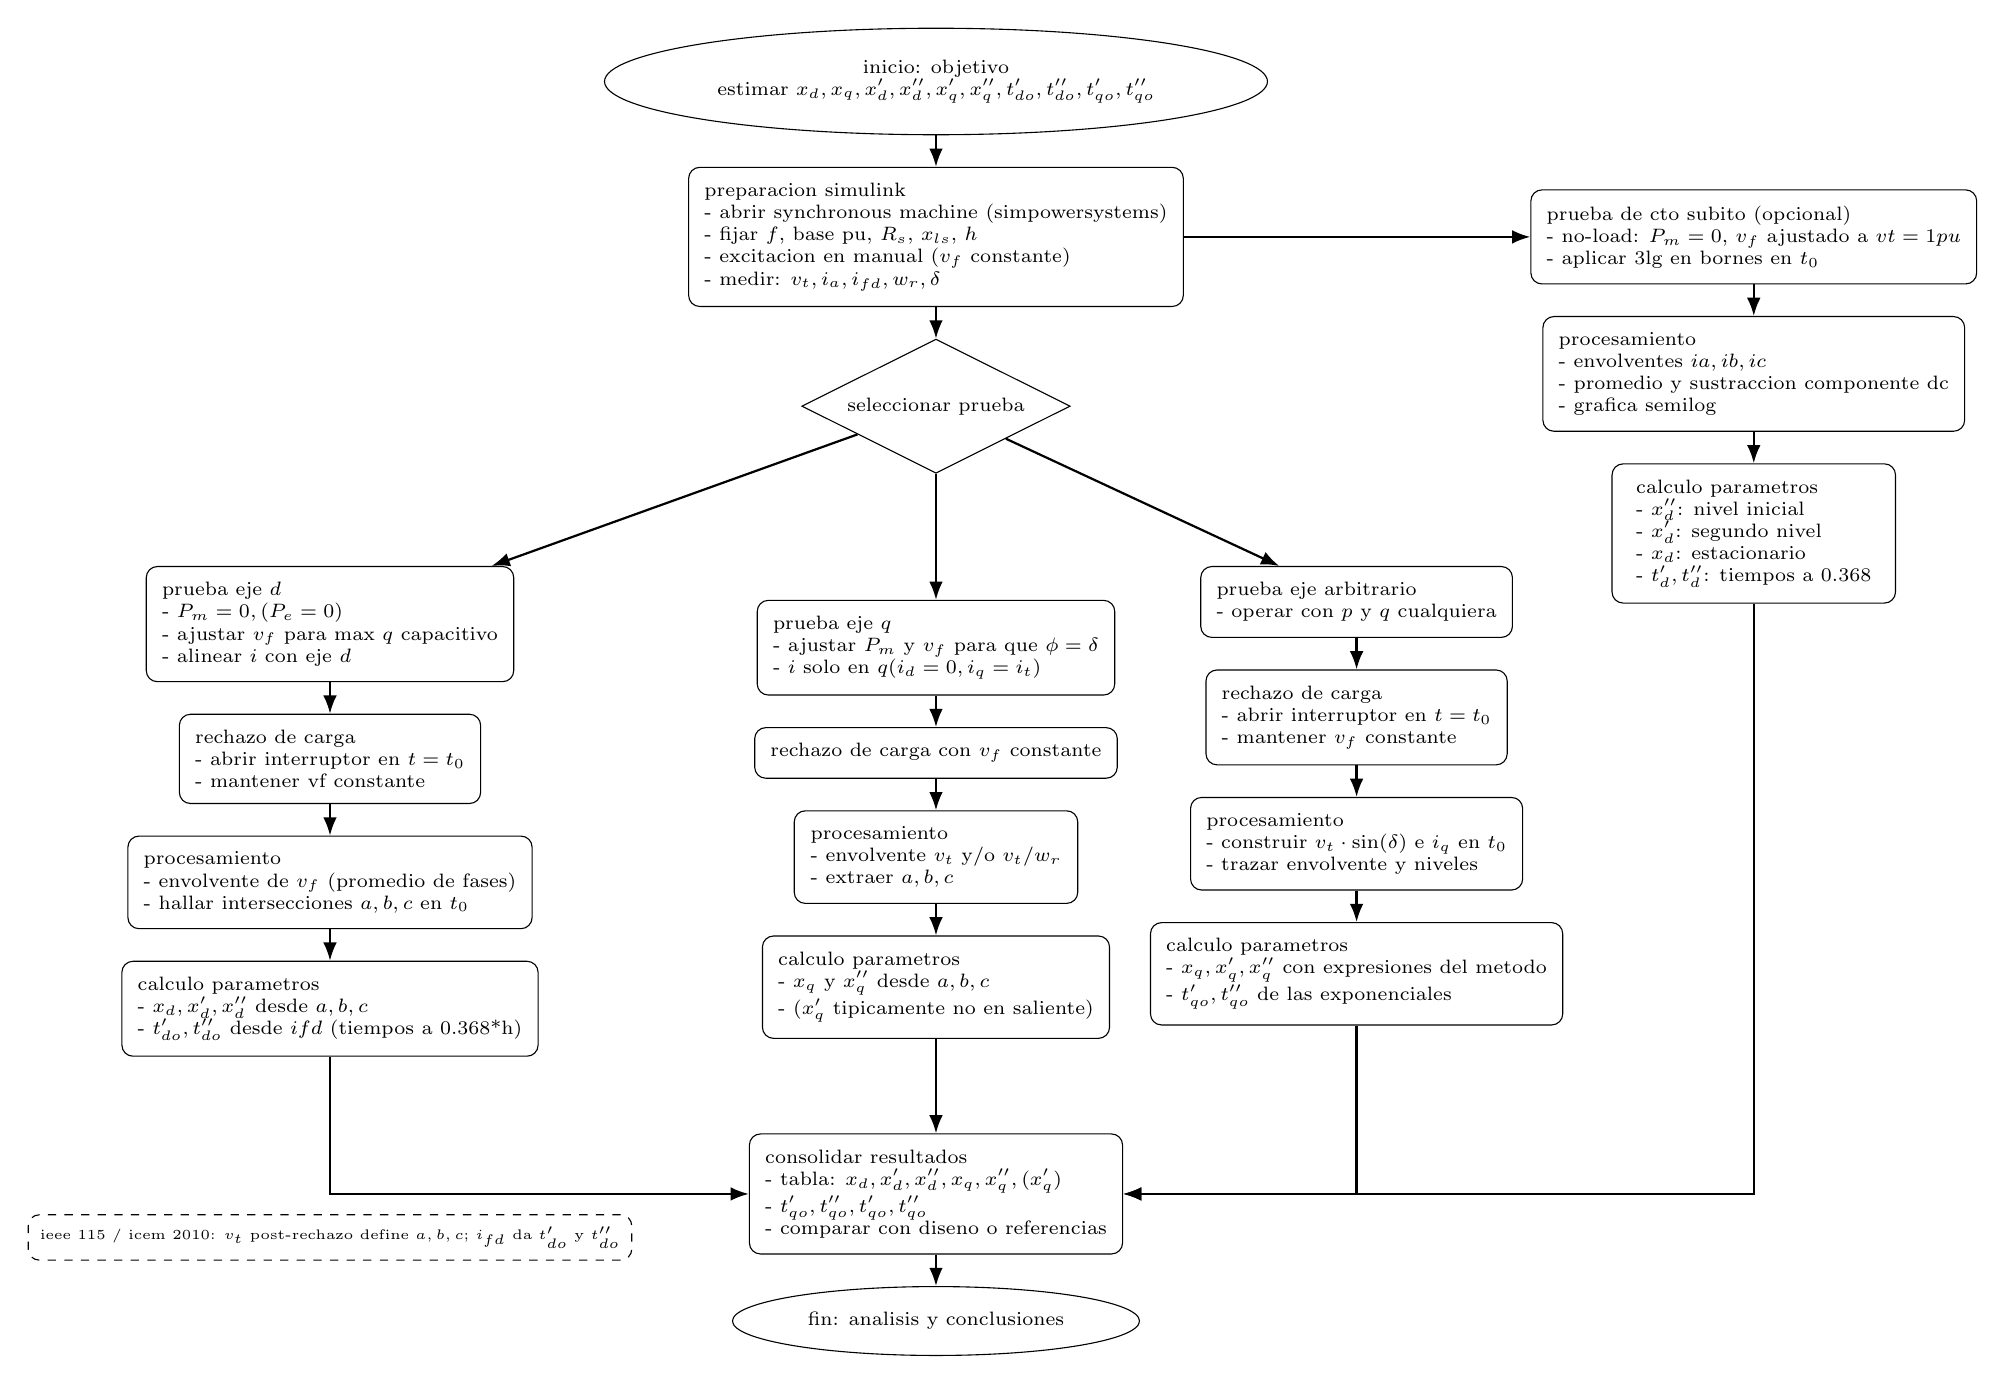
\begin{tikzpicture}[node distance=4mm and 4mm]

% ---- encabezado general ----
\node[startstop] (start) {inicio: objetivo\\
estimar $x_d, x_q, x'_d, x''_d, x'_q, x''_q, t'_{do}, t''_{do}, t'_{qo}, t''_{qo}$};

\node[box, below=of start] (prep) {preparacion simulink\\
- abrir synchronous machine (simpowersystems)\\
- fijar $f$, base pu, $R_s$, $x_{ls}$, $h$\\
- excitacion en manual ($v_f$ constante)\\
- medir: $v_t, i_a, i_{fd}, w_r, \delta$};

\node[dec, below=of prep] (branch) {seleccionar prueba};

% ---- rama d-axis (izquierda) ----
\node[box, below left=16mm and 45mm of branch] (dset) {prueba eje $d$\\
- $P_m = 0, (P_e = 0)$\\
- ajustar $v_f$ para max $q$ capacitivo\\
- alinear $i$ con eje $d$};
\node[box, below=of dset] (dtrip) {rechazo de carga\\
- abrir interruptor en $t = t_0$\\
- mantener vf constante};
\node[box, below=of dtrip] (dproc) {procesamiento\\
- envolvente de $v_f$ (promedio de fases)\\
- hallar intersecciones $a, b, c$ en $t_0$};
\node[box, below=of dproc] (dcalc) {calculo parametros\\
- $x_d, x'_d, x''_d$ desde $a,b,c$\\
- $t'_{do}, t''_{do}$ desde $ifd$ (tiempos a 0.368*h)};
\node[note, below=20mm of dcalc] (dref) {ieee 115 / icem 2010: $v_t$ post-rechazo define $a,b,c$; $i_{fd}$ da $t'_{do}$ y $t''_{do}$};

% ---- rama q-axis (centro) ----
\node[box, below=16mm of branch] (qset) {prueba eje $q$\\
- ajustar $P_m$ y $v_f$ para que $\phi = \delta$\\
- $i$ solo en $q (i_d = 0, i_q = i_t)$};
\node[box, below=of qset] (qtrip) {rechazo de carga con $v_f$ constante};
\node[box, below=of qtrip] (qproc) {procesamiento\\
- envolvente $v_t$ y/o $v_t/w_r$\\
- extraer $a,b,c$};
\node[box, below=of qproc] (qcalc) {calculo parametros\\
- $x_q$ y $x''_q$ desde $a,b,c$\\
- ($x'_q$ tipicamente no en saliente)};

% ---- rama arbitrary-axis (derecha) ----
\node[box, below right=16mm and 25mm of branch] (aset) {prueba eje arbitrario\\
- operar con $p$ y $q$ cualquiera};
\node[box, below=of aset] (atrip) {rechazo de carga\\
- abrir interruptor en $t = t_0$\\
- mantener $v_f$ constante};
\node[box, below=of atrip] (aproc) {procesamiento\\
- construir $v_t\cdot \sin(\delta)$ e $i_q$ en $t_0$\\
- trazar envolvente y niveles};
\node[box, below=of aproc] (acalc) {calculo parametros\\
- $x_q, x'_q, x''_q$ con expresiones del metodo\\
- $t'_{qo}, t''_{qo}$ de las exponenciales};

% ---- rama short-circuit (arriba derecha, opcional) ----
\node[box, right=44mm of prep] (scset) {prueba de cto subito (opcional)\\
- no-load: $P_m = 0$, $v_f$ ajustado a $vt = 1 pu$\\
- aplicar 3lg en bornes en $t_0$};
\node[box, below=of scset] (scproc) {procesamiento\\
- envolventes $ia, ib, ic$\\
- promedio y sustraccion componente dc\\
- grafica semilog};
\node[box, below=of scproc] (sccalc) {calculo parametros\\
- $x''_d$: nivel inicial\\
- $x'_d$: segundo nivel\\
- $x_d$: estacionario\\
- $t'_d, t''_d$: tiempos a 0.368};

% ---- consolidacion ----
\node[box, below=12mm of qcalc] (table) {consolidar resultados\\
- tabla: $x_d, x'_d, x''_d, x_q, x''_q, (x'_q)$\\
- $t'_{qo}, t''_{qo}, t'_{qo}, t''_{qo}$\\
- comparar con diseno o referencias};
\node[startstop, below=of table] (end) {fin: analisis y conclusiones};

% ---- conexiones ----
\draw[line] (start) -- (prep);
\draw[line] (prep) -- (branch);

\draw[line] (branch) -- (dset);
\draw[line] (dset) -- (dtrip);
\draw[line] (dtrip) -- (dproc);
\draw[line] (dproc) -- (dcalc);
\draw[line] (dcalc) |- (table);

\draw[line] (branch) -- (qset);
\draw[line] (qset) -- (qtrip);
\draw[line] (qtrip) -- (qproc);
\draw[line] (qproc) -- (qcalc);
\draw[line] (qcalc) -- (table);

\draw[line] (branch) -- (aset);
\draw[line] (aset) -- (atrip);
\draw[line] (atrip) -- (aproc);
\draw[line] (aproc) -- (acalc);
\draw[line] (acalc) |- (table);

\draw[line] (prep) -- (scset);
\draw[line] (scset) -- (scproc);
\draw[line] (scproc) -- (sccalc);
\draw[line] (sccalc) |- (table);

\draw[line] (table) -- (end);

\end{tikzpicture}%
}% end resizebox

\vspace{0.5ex}
\begin{minipage}{0.98\linewidth}\footnotesize
% notas rapidas (sin acentos)
notas:
(1) mantener vf constante y excitacion manual en todas las pruebas;
(2) eje $d$: $P_m=0$, ajustar $v_f$ hasta max q capacitivo; usar vt (promedio de fases) para a,b,c; ifd para t'do y t''do;
(3) eje $q$: ajustar $\phi = \delta (i_d=0)$ para $x_q$ y $x''_q$ de $a,b,c$;
(4) eje arbitrario: usar $v_t\cdot \sin(\delta)$ e $i_q$ en $t_0$ para $x_q$, $x'_q$, $x''_q$ y $t'_{qo}$, $t''_{qo}$;
(5) corto subitro: semilog de envolvente de corriente para x-values y tiempos 0.368.
\end{minipage}

\end{document}
